\documentclass[12pt]{article}

% --- Packages ---
\usepackage[utf8]{inputenc}
\usepackage[T1]{fontenc}
\usepackage[french]{babel}
\usepackage{amsmath, amssymb}
\usepackage{geometry}
\usepackage{tikz}
\usepackage[most]{tcolorbox}
\usepackage{multicol}
\usepackage{lmodern}
\usepackage{pgfplots}
\pgfplotsset{compat=1.18}
\usepackage{mdframed}
\usepackage{tkz-tab}
\usepackage{bm}
\usepackage{xcolor}
\usepackage{sectsty}
\usepackage[utf8]{inputenc}
\usepackage[T1]{fontenc}
\usepackage[inline]{enumitem}
\usepackage[dvipsnames]{xcolor}
\usepackage{multido}
% --- Page ---
\geometry{margin=2cm}

% Footer
\usepackage{fancyhdr}
\pagestyle{fancy}
\cfoot{\thepage}
\rfoot{\textit{G.M.}}
\renewcommand{\headrulewidth}{0pt}
\renewcommand{\footrulewidth}{0pt}

% Pour les normes : 
\newcommand*{\norme}[1]{\left\lVert\overrightarrow{#1}\right\rVert}

\usetikzlibrary{shapes.misc}

\tikzset{cross/.style={cross out, draw=black, minimum size=2*(#1-\pgflinewidth), inner sep=0pt, outer sep=0pt},
%default radius will be 1pt. 
cross/.default={4pt}}

% mettre dans le préambule, après \usepackage{xcolor}
\usepackage{sectsty} % gère facilement la couleur des titres
\setlength{\parindent}{0pt}

\sectionfont{\color{red}\Large\bfseries}     % pour \section*
\subsectionfont{\color{red}\large\bfseries\hspace{1cm}}

\begin{document}

% ============================
%   INÉQUATIONS
% ============================

\newpage

\begin{center}
    {\LARGE \textbf{Variations de fonctions}}\\[4mm]
    {\large Seconde}
\end{center}

\hrule
\vspace{0pt}

% ============================
%   PARTIE 1 : Inéquations du premier degré
% ============================

\section*{\textcolor{red}{Partie 1 : Fonctions croissantes et fonctions décroissantes}}

\subsection*{\hspace{1cm} 1) Définition}

On considère en exemple la fonction : $f(x) = 5x - x^2$

\vspace{10pt}
\begin{minipage}[t]{.45\textwidth}%
    \vspace{0pt}
    \begin{center}
        $f$ est \_\_\_\_\_\_\_\_\_\_\_\_ sur \_\_\_\_\_\_\_

        \vspace{10pt}
        Si $x$ augmente ({\color{red}1} < {\color{ForestGreen}2}),

        \vspace{10pt}
        $f(x)$ \_\_\_\_\_\_\_\_\_\_\_\_ (\_\_\_\_\_\_\_\_\_)
        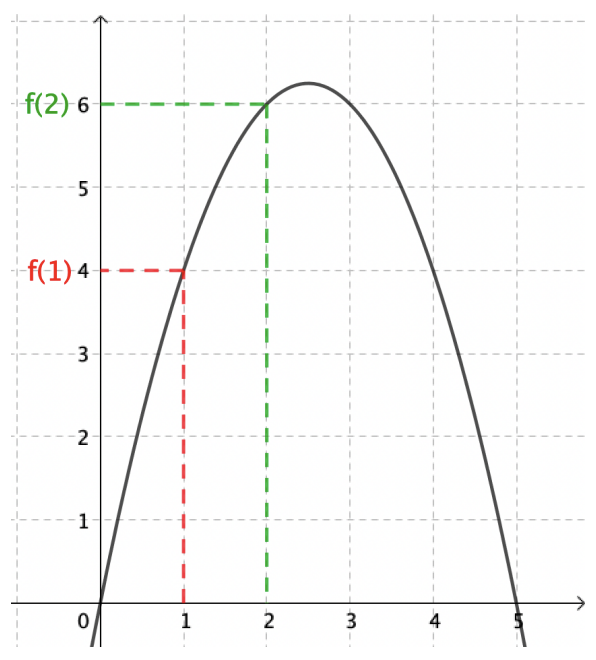
\includegraphics[width=0.8\textwidth]{var1.png}    
    \end{center}
\end{minipage}%
\hfill
\begin{minipage}[t]{.45\textwidth}%
    \vspace{0pt}
    \begin{center}
        $f$ est \_\_\_\_\_\_\_\_\_\_\_\_ sur \_\_\_\_\_\_\_

        \vspace{10pt}
        Si $x$ augmente ({\color{red}3} < {\color{ForestGreen}4}),

        \vspace{10pt}
        $f(x)$ \_\_\_\_\_\_\_\_\_\_\_\_ (\_\_\_\_\_\_\_\_\_)
        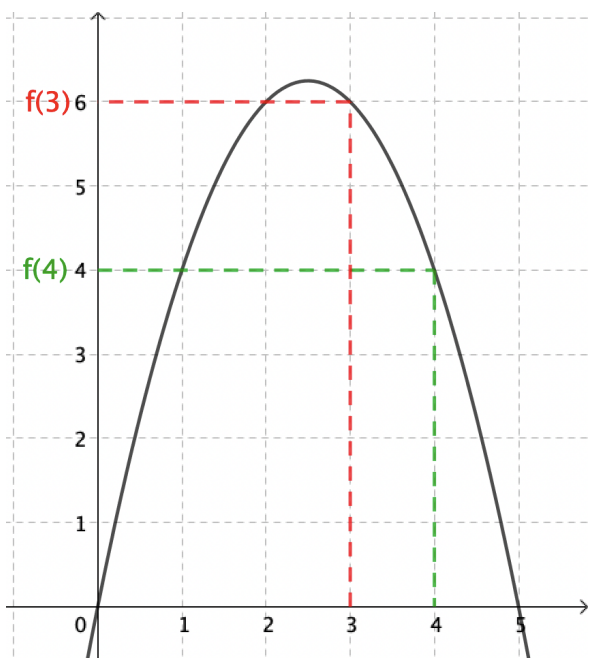
\includegraphics[width=0.8\textwidth]{var2.png}
    \end{center}
\end{minipage}%

\begin{mdframed}[
    linewidth=1pt,
    linecolor=ForestGreen,
    innertopmargin=10pt,
    innerbottommargin=10pt
]
{\color{ForestGreen}\textbf{\underline{Définition :}}}  
Sur une intervalle $I$,

\vspace{-5pt}
\begin{minipage}[t]{.45\textwidth}%
    \vspace{0pt}
    Une fonction $f$ est \textbf{croissante}, si $a < b$ alors $f(a) \leq f(b)$.
    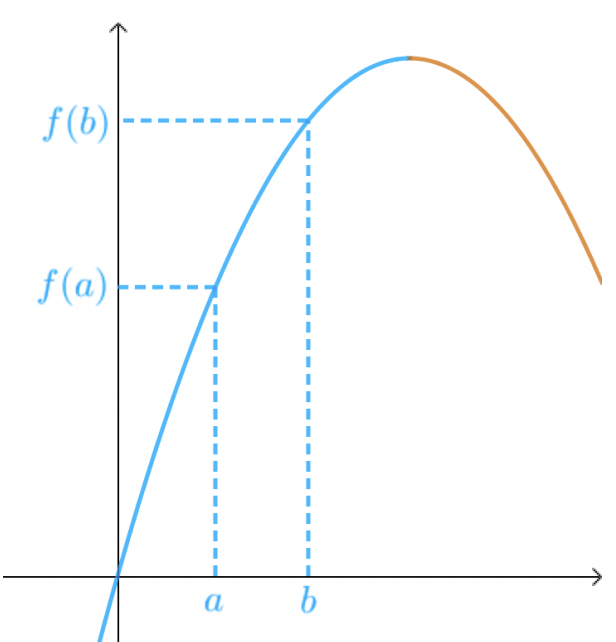
\includegraphics[width=0.8\textwidth]{vardef1.png}
\end{minipage}%
\hfill
\begin{minipage}[t]{.45\textwidth}%
    \vspace{0pt}
    Une fonction $f$ est \textbf{décroissante}, si $a < b$ alors $f(a) \geq f(b)$.
    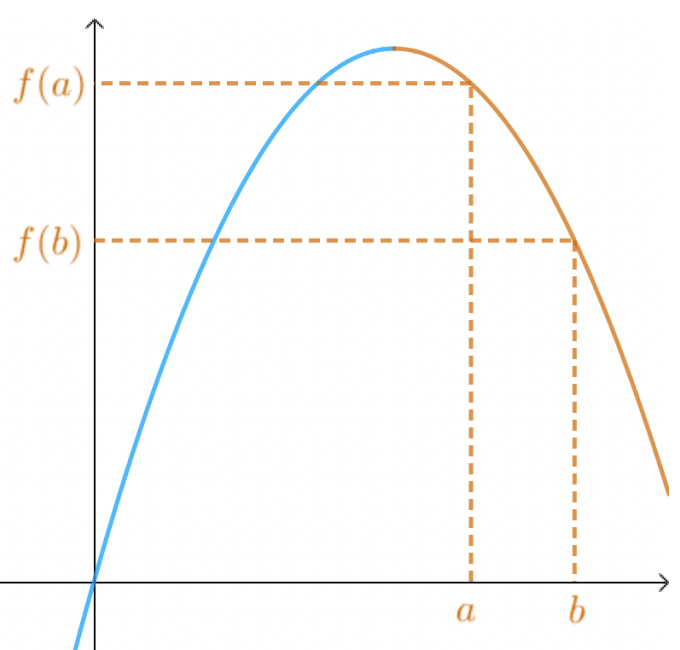
\includegraphics[width=0.8\textwidth]{vardef2.png}
\end{minipage}%
\end{mdframed}

\vspace{10pt}

\underline{Remarques :}
\begin{itemize}
    \item Pour une fonction $f$ \textbf{constante} : on a 
    toujours : \_\_\_\_\_\_\_\_\_\_\_\_.
    \item Dire que $f$ est monotone signifie que $f$ est \textbf{soit croissante soit décroissante}.
\end{itemize}

\vspace{5pt}

\begin{mdframed}[
    linewidth=1pt,
    linecolor=RoyalBlue,
    innertopmargin=10pt,
    innerbottommargin=10pt
]
{\color{RoyalBlue}\textbf{\underline{Exercice d'application n°1 :}}}
\vspace{10pt}

Décrire les variations de $g$ sur son ensemble de définition.

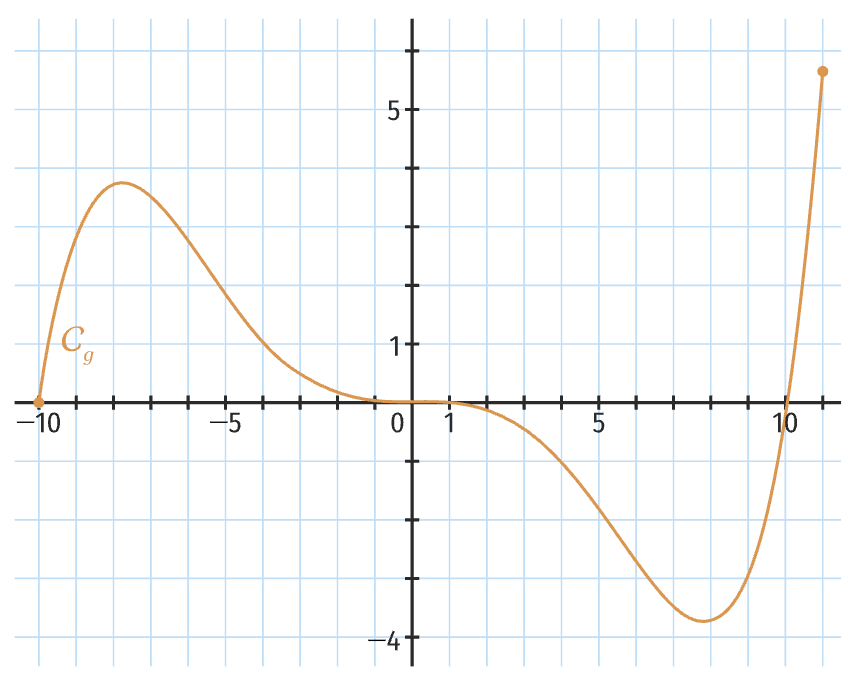
\includegraphics[width=0.6\textwidth]{exo1.png}
\end{mdframed}

\vspace{10pt}

% ========================================================
%             2) Maximum et minimum
% ========================================================
\subsection*{\hspace{1cm} 2) Maximum et minimum}

\vspace{5pt}
\underline{Exemple :}
Reprenon l'exemple de tout à l'heure avec $f(x) = 5x - x^2$.

\begin{minipage}[t]{.45\textwidth}%
    \vspace{15pt}
    Sur l’intervalle $\left[0 ; 5\right]$, on a :
    
    \vspace{15pt}
    $f(x) \leq $\ \ \_\_\_\_\_\_ $=$ \_\_\_\_\_\_.

    \vspace{15pt}
    On dit que \_\_\_\_\_\_ est le 
    
    \vspace{15pt}
    \_\_\_\_\_\_\_\_\_\_\_\_ de la fonction $f$.

    \vspace{15pt}
    Ce \_\_\_\_\_\_\_\_\_\_\_\_ est atteint en 
    
    \vspace{15pt}
    \_\_\_\_\_\_.
\end{minipage}%
\hfill
\begin{minipage}[t]{.45\textwidth}%
    \vspace{0pt}
    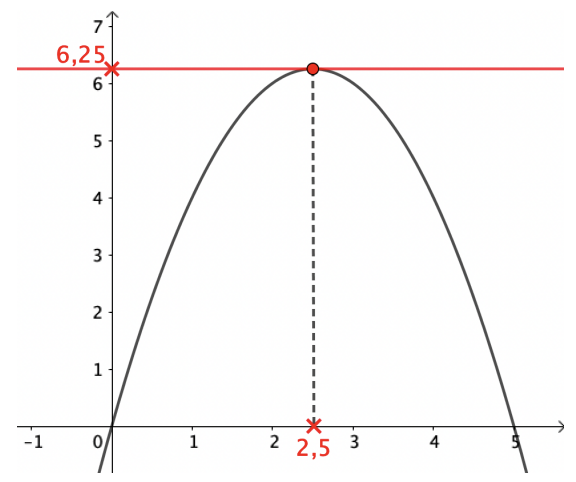
\includegraphics[width=1\textwidth]{exemple2.png}
\end{minipage}%

\begin{mdframed}[
    linewidth=1pt,
    linecolor=ForestGreen,
    innertopmargin=10pt,
    innerbottommargin=10pt
]
{\color{ForestGreen}\textbf{\underline{Définition :}}}  
Sur une intervalle $I$,

\vspace{5pt}
\begin{minipage}[t]{.45\textwidth}%
    \vspace{10pt}
    \begin{itemize}
        \item Une fonction $f$ admet un \textbf{maximum} $M$ en $a$, si pour tout $x$,
        \\$f(x) \leq f(a) = M$.

        \vspace{20pt}
        \item Une fonction $f$ admet un \textbf{minimum} $m$ en $b$, si pour tout $x$,
        \\$f(x) \geq f(b) = m$.
    \end{itemize}
\end{minipage}%
\hfill
\begin{minipage}[t]{.45\textwidth}%
    \vspace{-30pt}
    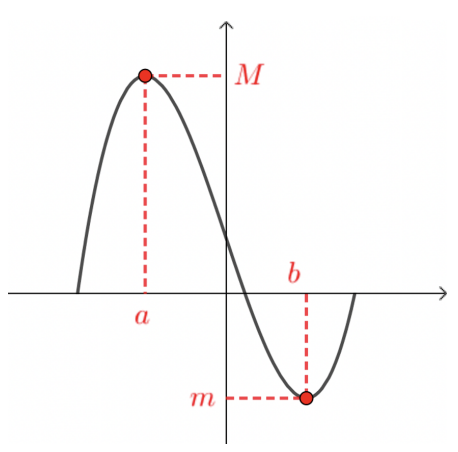
\includegraphics[width=0.8\textwidth]{defmaxmin.png}
\end{minipage}%
\end{mdframed}

\vspace{10pt}
\underline{Remarque :}
Un minimum ou un maximum s'appelle un \_\_\_\_\_\_\_\_\_\_\_\_.

\vspace{20pt}

% ========================================================
%             3) Tableau de variations
% ========================================================
\subsection*{\hspace{1cm} 3) Tableau de variations}

\vspace{5pt}
\underline{Méthode :} Déterminer graphiquement les variations d'une fonction et dresser le tableau de 
variations.

\vspace{5pt}
On considère la représentation graphique de $f$ suivante : 

\begin{center}
    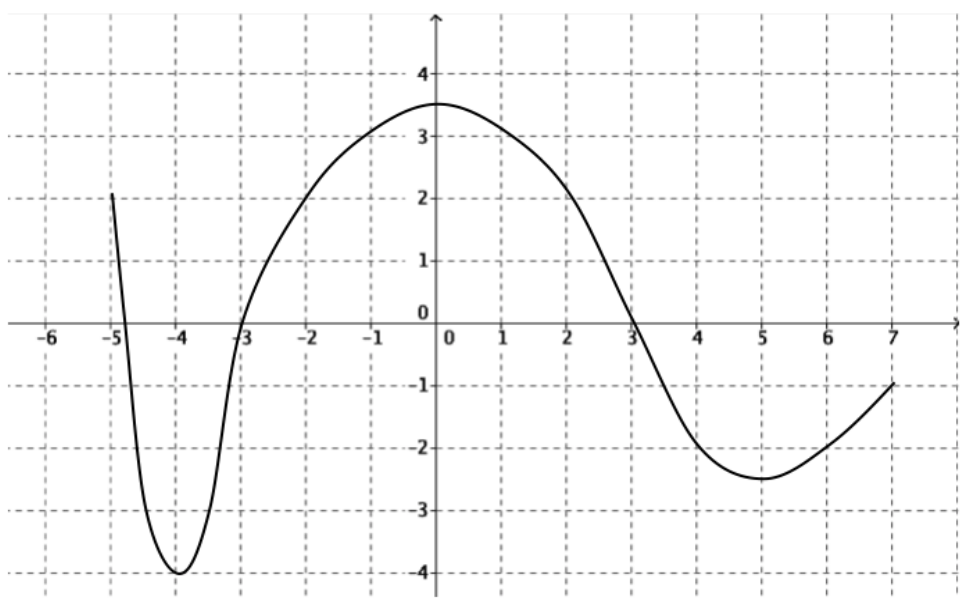
\includegraphics[width=0.8\textwidth]{exo2.png}    
\end{center}

\vspace{20pt}
La fonction $f$ est définie sur \_\_\_\_\_\_\_\_\_\_\_\_.

\vspace{20pt}
La fonction $f$ est \_\_\_\_\_\_\_\_\_\_\_\_ sur les intervalles \_\_\_\_\_\_\_\_\_\_\_\_ et \_\_\_\_\_\_\_\_\_\_\_\_.

\vspace{20pt}
Elle est \_\_\_\_\_\_\_\_\_\_\_\_ sur les intervalles \_\_\_\_\_\_\_\_\_\_\_\_ et \_\_\_\_\_\_\_\_\_\_\_\_.

\vspace{20pt}
Le maximum de $f$ est \_\_\_\_\_\_. Il est atteint en \_\_\_\_\_\_\_\_\_.

\vspace{20pt}
Le minimum de $f$ est \_\_\_\_\_\_. Il est atteint en \_\_\_\_\_\_\_\_\_ .

\vspace{20pt}
Le tableau de variation de $f$ est le suivant :
\[
\begin{tikzpicture}
    \tkzTabInit{$x$ / 1 , $f(x)$ / 2.5}
    {,,,,}
    \tkzTabLine{}
\end{tikzpicture}
\]

\vspace{20pt}
% ========================================================
%             Partie 2 : Cas des fonctions affines
% ========================================================
\section*{\textcolor{red}{Partie 2 : Cas des fonctions affines}}

% ========================================================
%             1) Définitions
% ========================================================
\subsection*{\hspace{1cm} 1) Définitions}

\begin{mdframed}[
    linewidth=1pt,
    linecolor=ForestGreen,
    innertopmargin=10pt,
    innerbottommargin=10pt
]
{\color{ForestGreen}\textbf{\underline{Définition :}}}  
Une fonction affine $f$ est définie sur $\mathbb{R}$ par $f(x) = ax+b$, où $a$ et $b$ sont deux
nombres réels.

\vspace{5pt}
Lorsque $b$ = 0, la fonction $f$ définie par $f(x) = ax$ est une fonction \_\_\_\_\_\_\_\_\_\_\_\_.
\end{mdframed}

% ========================================================
%             2) Variations
% ========================================================
\subsection*{\hspace{1cm} 2) Variations}

\begin{mdframed}[
    linewidth=1pt,
    roundcorner=5pt,
    linecolor=Red,
    innertopmargin=10pt,
    innerbottommargin=10pt
]
{\color{red}
\underline{Propriété :} \textbf{Taux d'accroissement d'une fonction affine}

\vspace{5pt}
Soit $f$ une fonction affine définie sur $\mathbb{R}$ par $f(x) = ax+b$.
\begin{itemize}
    \item Si $a>0$, alors $f$ est croissante
    \item Si $a<0$, alors $f$ est décroissante
    \item Si $a=0$, alors $f$ est constante
\end{itemize}
}
\end{mdframed}

\underline{Méthode :}
Considérons trois fonctions $f$, $g$ et $h$ suivantes :

\begin{minipage}[t]{.25\textwidth}%
    \vspace{0pt}
    $f(x) = 3x + 2$

    \vspace{15pt}
    $g(x) = 7 - 7x$

    \vspace{15pt}
    $f(x) = -x$
\end{minipage}%
\hfill
\begin{minipage}[t]{.75\textwidth}%
    \vspace{0pt}
    $f$ est \_\_\_\_\_\_\_\_\_\_\_\_ car \_\_\_\_\_\_\_\_\_

    \vspace{15pt}
    $g$ est \_\_\_\_\_\_\_\_\_\_\_\_ car \_\_\_\_\_\_\_\_\_

    \vspace{15pt}
    $h$ est \_\_\_\_\_\_\_\_\_\_\_\_ car \_\_\_\_\_\_\_\_\_
\end{minipage}%



\end{document}
